\documentclass[12pt]{article} % Default font size is 12pt, it can be changed here
\usepackage{geometry} % Required to change the page size to A4
\geometry{a4paper,left=2cm,right=2.0cm,top=2.5cm,bottom=2.5cm} % Set the page size to be A4 as opposed to the default US Letter
\usepackage[toc,page]{appendix}
\usepackage{graphicx} % Required for including pictures
\usepackage{booktabs}
\usepackage{float} % Allows putting an [H] in \begin{figure} to specify the exact location of the figure
\usepackage{wrapfig} % Allows in-line images such as the example fish picture
\usepackage{fancyhdr}
\usepackage{lipsum} % Used for inserting dummy 'Lorem ipsum' text into the template
\usepackage{lastpage}
\usepackage[ruled,vlined]{algorithm2e}
\usepackage{caption}
\usepackage{subfigure}
\usepackage{palatino}
\usepackage[table,xcdraw]{xcolor}
\usepackage{enumerate}
\usepackage{verbatim}

\linespread{1.0} % Line spacing
\graphicspath{{Pictures/}} % Specifies the directory where pictures are stored
\pagestyle{fancy}
\begin{document}
	\lhead{Team \# 1901279}
\rhead{Page \thepage \ of \pageref{LastPage}}
\cfoot{}
\thispagestyle{fancy}
\begin{center}
{\LARGE Who Drugged Me? }
\end{center}

\tableofcontents % Include a table of contents
\newpage % Begins the essay on a new page instead of on the same page as the table of contents 

\section{Introduction} % Major section
\subsection{Problem Background} % Sub-section
[Problem Background] see in problem background.tex

\subsection{Our Work} % Sub-section
[Our Work] See in OurWork.tex

\begin{equation}
E=mc^2+\sqrt{E}
\end{equation}

\section{Assumptions and Notations} % Major section
\subsection{Assumptions}
[Assumptions] see file Assumptions.tex

\subsection{Notations} % Major section
[Notations] see in Notations.tex

%-------------------------------
The following variables will be defined here here as they are widely used throughout this paper. Additional variables might be defined later, but restricted to a particular section.

\begin{table}[H]
	\centering
	\begin{tabular}{|c|c|}
		\hline
		\rowcolor[HTML]{656565} 
		{\color[HTML]{FFFFFF} \textbf{Symbol}} & {\color[HTML]{FFFFFF} \textbf{Definition}} \\ \hline
		i    & the $i_{th}$ item in a series of unsigned integer numbers  \\ \hline
		i    & the $i_{th}$ item in a series of unsigned integer numbers  \\ \hline
		i    & the $i_{th}$ item in a series of unsigned integer numbers  \\ \hline
		i    & the $i_{th}$ item in a series of unsigned integer numbers  \\ \hline
		i    & the $i_{th}$ item in a series of unsigned integer numbers  \\ \hline
	\end{tabular}
	\caption{Notations}
\end{table}

\section{Data Processing}
Upon investigation, we find that the data in \textit{MCM\_NFLIS\_Data.xlsx} is already in desired form. Therefore we shall mainly focus on the data processing for  \textit{ACS\_XX\_5YR.xlsx}

There are three main types of missing data mechanisms: Missing Completely at Random(MCAR), Missing at Random(MAR) and Missing not at random(NMAR). Upon investigation, we find that 

\begin{enumerate}[\bfseries Problem 1.]
	\item Missing data in the form of "**", "-", "(X)" and so on.
	\item Tags may vary in description between different years, for example in some datasets, the tag \textit{Total Households} is used, while in others \textit{Total households} and \textit{Family Households} is used, making it difficult for automatic comparison.
	\item Certain tags disappear in some years, and reappear in others. 
	\item The counties that appeared in ACS datasets and NFLIS datasets are not always unanimous.
\end{enumerate}

First we address with the missing data problem, which mainly appear in file.

\begin{enumerate}[\bfseries Step 1.]
	\item For each ACS\_xx\_5YR\_DP02.csv file, we separate the \textit{data area} with others. The \textit{data area} includes only digits, "*", "-" and "(X)". 
	\item We remove all columns in the \textit{data area} with more than ten "(X)" values.
	\item We've just evacuated the missing data in the \textit{data area} with  "*", "-" or "(X)".
	\item Remove all factor columns which did not appear all through year 2010-2016.
\end{enumerate}


\section{Model Overview} % Sub-section
\subsection{the Continuum Drug Spread Model}
Our model is inspired by the Porous Media Contaminant Transport Model.\cite{8} The transport process is expressed in a differential equation, balancing the total mass of contaminant in the fracture. 

Similarly, we propose a Continnum Drug Spread(CDS) model. This model, which is expressed in a \textbf{\itshape partial differential equation}, is constructed under the assumption that we view the geographical features in a continuous way. 

Let $S(x,y,t)$ represent the amount of drug stored in $(x,y)$ at time $t$. The NFLIS data contains drug identification counts in years 2010-2017 for narcotic analgesics and heroin in each of the counties from the five states stated in the \textit{problem background} section, which we denote as $F(x,y,t)$, the amount of drugs identified in $(x,y)$ at time $t$. We assume that the amount of identified drugs is directly proportional to the total amount of drugs with a proportionality constant $k$, such that
\begin{equation}
S(x,y,t) = k\cdot F(x,y,t)
\end{equation}

We denote the total amount of drug used in $(x,y)$ at time $t$ with $U(x,y,t)$, and since the amount of drug used is less or equal to the amount of drug stored in the same location at the same time, we have
\begin{equation}
U(x,y,t) = \lambda S(x,y,t), 0\leq \lambda \leq 1
\end{equation}

It is natural to assume that $\lambda$ is revelant with socio-economical factors of the given location. We shall address this in the second part of the problem.

Intuitively, $D(\frac{\partial^2 S}{\partial x^2} + \frac{\partial^2 S}{\partial y^2})$ can be used to describe the total amount of drug transported into the city. $\frac{\partial^2 S}{\partial x^2} + \frac{\partial^2 S}{\partial y^2}$ describes the \textit{emergency} of transporting drugs, i.e. the trend of transporting drug from $(x,y)$ to neighboring coordinates.

The difference between the total amount of drug transported into $(x,y)$ and the amount of drug used equals to the change of storage:

\begin{equation}
D(\frac{\partial^2 S}{\partial x^2} + \frac{\partial^2 S}{\partial y^2}) - \lambda S = \frac{\partial S}{\partial t} 
\end{equation}

$S$, however, is unknown. We substitute (1) into (3), and eliminate the common factor $k$ from both sides of the equation
\begin{equation}
D(\frac{\partial^2 F}{\partial x^2} + \frac{\partial^2 F}{\partial y^2}) - \lambda F = \frac{\partial F}{\partial t}
\end{equation}

\subsection{Analytical Solution to the CDS Model}

\subsection{Identify the Origin of Specific Opioid Use}
We compose a 3D image describing the characteristics of the reported synthetic opioid and heroin cases across counties. We transform the FIPS coding of the counties into their latitude and longitude. The x-axis represents the latitude, the y-axis represents the longitude, and the z-axis represents the specific drug reports.

We comopose a continuous 3D model of the latitude-longitude-drugreport relationship using quadratic interpolation. According to our assumption(A1-2), a Producer of a specific opioid use should reach a local maxima in drug reports. An Origin, which is a subset of Producers, possess the same statistical feature. A contour map(Figure 1(a)) is composed to visualize this ideology.

\begin{figure}[H]
	\centering
	\subfigure[3D Plot]{
		\centering
		\begin{minipage}[t]{0.3\linewidth}
			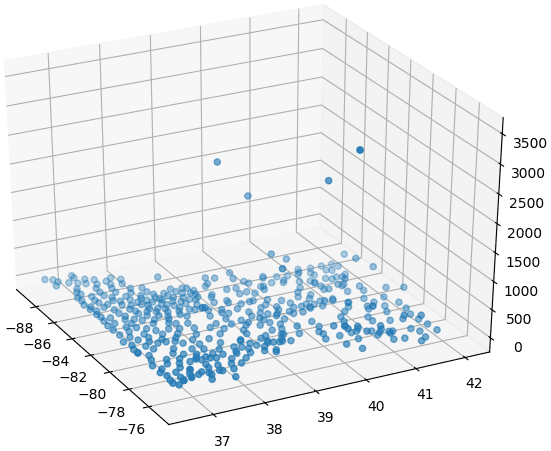
\includegraphics[width=2in]{001}
		\end{minipage}
	}
	\subfigure[Contour Map]{
		\centering
		\begin{minipage}[t]{0.4\linewidth}
			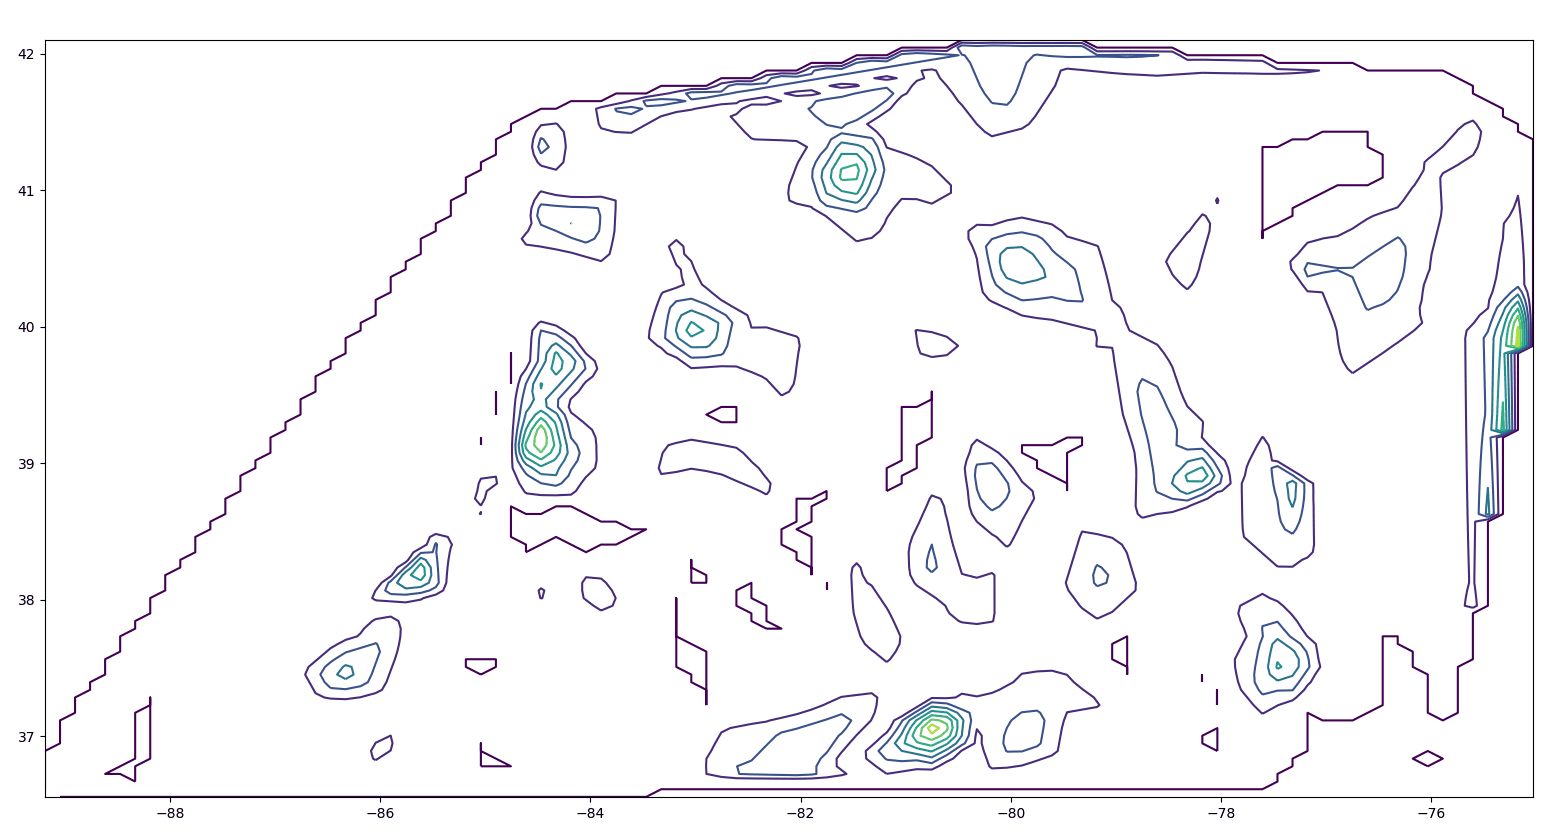
\includegraphics[width=3in]{000}
		\end{minipage}
	}
	\caption{Heroin}
\end{figure}

As illustrated in A3, not all Producers are Origins. Therefore, not all local maximum indicate Origins. We need to set up a threshold to distinguish Producers from Origins. 

Therefore, we identify the possible locations where specific opioid use might have started by computing all local maxima(see algorithm 1), and rank them to find the possible origins in each of the five states. The details of our ranking scheme concerns a comparison of a certain county's data in time. If a county remains a Producer(i.e. local maxima) for six years in a row, then we define it as a \textbf{\itshape Potential Origin}. For each state, if the number of Potential Origins is greater than 3, then we select three Potential Origins with top three specific opioid reports as the possible Origins for the opioid in discussion of that state.



\subsection{Drug Identification Threshold}
We endeavor to propose a drug identification threshold such that when a county's total opioid report reaches this threshold, the U.S. government should be extremely concerned with opioid control in this county.

Statistics from the dataset reveal that on average, 92 cases of opioid identifications occur in a county per year. Traversing the map, we find that in counties with severe drug crisis, thousands of opioid identification may occur per year. Under this premesis, we classify the Producers into three levels(see Table 2).

\begin{table}[H]
	\centering
	\begin{tabular}{|c|c|}
		\hline
		\rowcolor[HTML]{656565} 
		{\color[HTML]{FFFFFF} \textbf{Level}} & {\color[HTML]{FFFFFF} \textbf{Threshold}} \\ \hline
		First-Level Origin  & total Drug Report per year $\geq 1000$ \\ \hline
		Second-Level Origin & $100 \leq$ total Drug Report per year $\leq 1000$ \\ \hline
		Third-Level Origin  & total Drug Report per year $\leq 100$ \\ \hline
	\end{tabular}
	\caption{Notations}
\end{table}

These three levels indicate the degree at which the U.S. government need to be alarmed. First level origins are counties with severe opioid crisis. Third-level origins are those with minor opioid crisis. The second level is in-between.

The strategy against different level of origins vary. First level origins require immediate control and intervention, while third level origins could be treated with a mild approach. For origins in the second level, the government need to focus specifically on those in danger of transforming from the second to the first level.

\subsection{Model Prediction via the Grey Method}
The database provides us with the record of total drug identification cases from 2010 to 2017. We could use Grey Method to predict the future data based on our current model.

The Gray Model is applied mainly on incomplete data and undeterminable problems. We the use GM(1,1) model for prediction.\cite{13}

Let $X$ be a sequence of observed data, such that
\begin{equation}
X^{(0)} = (X^{(0)}(1),X^{(0)}(2),\cdots,X^{(0)}(n))
\end{equation}
Here, $X^{(0)}(i)$ represents the observed data at time $i$. We generate the first-order Accumulated Generating Operation sequence  $X^{(1)}(i)$ based on $X^{(0)}(i)$, where
\begin{equation}
X^{(1)}(i) = \sum_{k=1}^i X^{(0)}(k) = X^{(1)}(i-1)+X^{(0)}(i)
\end{equation}
Then we establish the first-order differential equation of $X^{(1)}(i)$ as
\begin{equation}
\frac{dX^{(1)}}{dt}+aX^{(1)}=u
\end{equation}
where $a$ and $u$ are parameters we wish to obtain. (6) and (7) reveal that
\begin{equation}
\hat{X}^{(1)}(i+1) = (X^{(0)}(1)-\frac{u}{a})e^{-ai}+\frac{u}{a}
\end{equation}
Now we attempt to fit parameter $a$ and $u$, as described in (7). Let $\hat{a}$ be a sequence of parameters where $\hat{a}=[a,u]^T$. The solution to $\hat{a}$ is
\begin{equation}
\hat{a} = (B^T B)^{-1}B^TY_n
\end{equation}
where
\begin{equation}
B=\left[
\begin{array}{cc}
-\frac{1}{2}[X^{(1)}(1)+X^{(1)}(2)] & 1\\
-\frac{1}{2}[X^{(1)}(2)+X^{(1)}(2)] & 1\\
\cdots & \cdots \\
-\frac{1}{2}[X^{(1)}(n-1)+X^{(1)}(n)] & 1\\
\end{array}
\right],
Y_n = [X^{(0)}(2),X^{(0)}(3),\cdots, X^{(0)}(n)]^T
\end{equation}








\section{Analysis on Socio-Economic Factors} \subsection{Initializing the Directed Graph}
In the original Opoid Spread Model, we temporarily overlooked the relationship between the parameter $\lambda$ and position $(x,y)$ in the formula. In this section, we modify our model to reveal the relationship between $\lambda$ and local socio-economic factors. 

Using the same algorithm introduced for locating the Possible Origin of specific opioid(see 4.3), we discovered the following seven Possible Origins for general Opioids.

\begin{table}[H]
	\centering
	\begin{tabular}{|c|c|c||c|c|c|}
		\hline
		\rowcolor[HTML]{656565} 
		{\color[HTML]{FFFFFF} \textbf{STATE}} & {\color[HTML]{FFFFFF} \textbf{COUNTY}} & {\color[HTML]{FFFFFF} \textbf{F}} &{\color[HTML]{FFFFFF} \textbf{STATE}} & {\color[HTML]{FFFFFF} \textbf{COUNTY}} & {\color[HTML]{FFFFFF} \textbf{F}}\\ \hline
		KY & - & - &OH & Mahoning & 2115 \\ \hline
		VA & - & - &OH & Cuyahoga & 12190\\ \hline
		WV & - & - &OH& Lake &3003 \\ \hline
		OH & Hamilton & 11896 &PA & Philadelphia & 23431 \\ \hline
		OH & Stark & 2539 & PA & Allegheny & 8268 \\ \hline
	\end{tabular}
	\centering
	\caption{Possible Origins of Opioids in General}
\end{table}

Since detailed information concerning opoid amount is limited, and the properties of $\lambda$ differ regarding whether the county is a Source or a Consumer , we need to make the following assumptions to simplify our model in order to estimate the value of $\lambda$:

\begin{enumerate}
	\item For Consumers, $\lambda \approx 1$. This indicates that Consumers have a limited ability to transport drugs into neighboring counties, and can be omitted when conducting simplified calculations.
	
	\item Based on the above assumption, we can estimate $\lambda$ for Sources by
	\begin{equation}
	\lambda_{Source_i}=\frac{F_{Source_i}}{F_{Source_i}+\sum_{j\in N_i} F_{Consumer_j}}
	\end{equation} 
\end{enumerate}

\textit{
NOTE: In the following analysis, we abbreviate $\lambda_{Source_i}$ to $\lambda_i$, since we will mainly be considering the $\lambda$ value for Sources, and therefore no confusion shall occur. 
}

\begin{figure}[H]
	\centering
	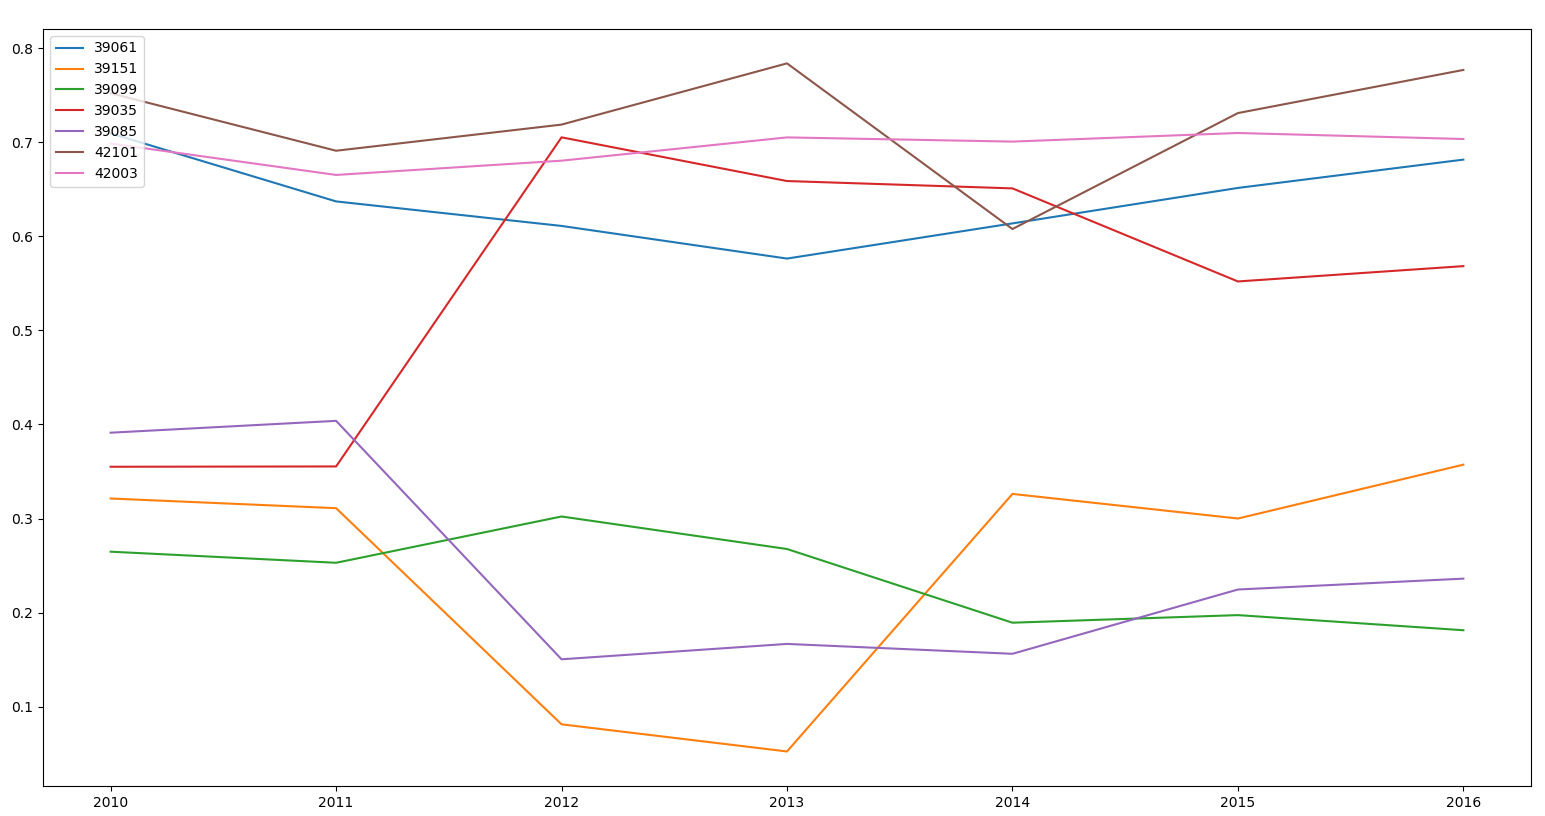
\includegraphics[width=0.6\linewidth]{004}
	\caption{$\lambda$ for the Possible Origins of Opioids in General over Time}
\end{figure}

We computed $\lambda$ for the seven Possible Origins during 2010-2016(see Figure 2). In order to eliminate the negative effect that a steep variation might cause, we calculate $\overline{\lambda_i}$, which is the average $\lambda$ for the $i_{th}$ Possible Origin through 2010-2016:

\begin{table}[H]
	\centering
\begin{tabular}{|c|c|c|c|c|c|c|c|}
	\hline
	\rowcolor[HTML]{656565} 
	{\color[HTML]{FFFFFF} \textbf{SOURCE(FIPS Code)}} &{\color[HTML]{FFFFFF} \textbf{39061}} & {\color[HTML]{FFFFFF} \textbf{39151}} & {\color[HTML]{FFFFFF} \textbf{39099}}  & {\color[HTML]{FFFFFF} \textbf{39035}} & {\color[HTML]{FFFFFF} \textbf{39085}} & {\color[HTML]{FFFFFF} \textbf{42101}}  & {\color[HTML]{FFFFFF} \textbf{42003}}\\ \hline
	$\overline{\lambda}$ & 0.6401 & 0.2499 & 0.2365 & 0.5492 & 0.2470 & 0.7231 & 0.6948 \\ \hline
\end{tabular}
\centering
\caption{$\overline{\lambda_i}$ for the Seven Possible Origins}
\end{table}

As we can see in the table above, the $\overline{\lambda_i}$ obviously vary among the Possible Origins. We have
\begin{equation}
\hat{\lambda}=\frac{\sum_{t=1}^{7}\overline{\lambda_i}}{7}=0.4773
\end{equation}
which indicates the average level of $\overline{\lambda_i}$, then we compute the difference of each $\overline{\lambda_i}$ from average.
\begin{equation}
\Delta \overline{\lambda_i} = \overline{\lambda_i} - \hat{\lambda}
\end{equation}
Our purpose here is to analyze which socio-economic factors contributed to such differences.

\subsection{Prior Knowledge}
The ACS dataset provided more than five hundred possible factors, so feature extraction is obviously needed. 

A series of hypothesis have been developed to explain the socio-economic factors related to opioid use. Basing on statistics summarized by the American Addiction Center and other institutes\cite{10}\cite{11}, we obtain the following information:
\begin{itemize}
	\item \textbf{EDUCATION.} College graduates aged 26 or older battled opoid addiction at lower rates than those who did not graduate from high school or those who didn’t finish college.
	\item \textbf{LONELINESS.} Those who live alone cope with opoid addiction more than those who don't.
	\item \textbf{DISABILITY.} Those with a disability are more likely to be treated with opiods and thus more likely to become addicted.
	\item \textbf{GENDER/RACE.} Contradictory reports exist on the influence of gender and entity/race on obtaining opoid addiction. 
	\item \textbf{POVERTY/UNEMPLOYMENT/FAMILY HISTORY.} Poverty, unemployment and family history are known risk factors of opioid misuse.
\end{itemize}


\begin{comment}
he above prior knowledge imply that education, loneliness, poverty, unemployment and family addiction history are the most influential factors. Contradicting reports regarding gender and entity factors allow us to assume that they play a minor part in opioid use.

Correspondingly, in the dataset, we choose \textit{\bfseries HC03\_VC85}(low educational background), \textit{\bfseries HC03\_VC14}(Nonfamily households - Householder living alone) and \textit{\bfseries HC01\_VC103}(DISABILITY STATUS OF THE CIVILIAN NONINSTITUTIONALIZED POPULATION - Total Civilian Noninstitutionalized Population). Let them be $Y_1$, $Y_2$ and $Y_3$ Further investigation showed that \textit{\bfseries HC01\_VC103} and all other disability-relevant factors were missing and therefore removed in the data cleansing proceidure. Therefore, we attempt to obtain $\lambda$ through linear regression by fitting
\begin{equation}
\lambda = \beta_1 Y_1 + \beta_2 Y_2
\end{equation}
\subsubsection{Linear Regression}
\end{comment}



%-------------------------------------

\subsection{Feature Extraction via LASSO}
We do not rely directly on prior knowledge to extract features related to $\lambda$. In order to derive useful information from the dataset, we use the LASSO method to roughly observe how each factor contributes to $\lambda$. 

Suppose that there are $N$ counties in the dataset, and each of these counties consists of $p$ covariates(i.e. socio-economic factors). We map these covariates to the corresponding total opoid use. In otherwords, the total opoid use is denoted as the \textbf{ \itshape outcome}. Let $y_i$ be the outcome(i.e. $F_i(x,y)$ in this context) and $x_i = (x_1, x_2, \cdots, x_p)^T$ be the covariate vector for the $i_{th}$ case.

To guarantee the reliability of the data, we removed all margin errors and some other redundant features including ANCESTRY, LANGUAGE, YEAR OF ENTRY and PLACE OF BIRTH. More details were discussed in section 3, Addressing Missing Data.

The LASSO estimate is defined by\cite{7}
\begin{equation}
\hat{\omega}_{LASSO}=
\arg\min_{\omega} \sum_{i=1}^{N}(y_i - x_i^T\omega)^2 + \theta||\omega||_1
\end{equation}

subject to
\begin{equation}
 \sum_{j=1}^{p}|\omega_j|\leq t
\end{equation}

Here, $t$ determines the level of regularization, and $\omega$ the weight. We fit the model using the coordinate descent algorithm. \cite{6}

We set the penalty factor $\theta$ to 1 to maximize the reduction in dimensions and extract the most valuble and relevant feature correlated with opoid use. The LASSO result of five most influential features and their weights is shown in Table 11.

\begin{table}[H]
	\centering
	\begin{tabular}{|l|l|}
		\hline
		\rowcolor[HTML]{656565} 
		{\color[HTML]{FFFFFF} \textbf{FEATURE}} & {\color[HTML]{FFFFFF} \textbf{WEIGHT}} \\ \hline
		
		Estimate; SCHOOL ENROLLMENT - 	&2083.42 \\ 
		High school (grades 9-12) & \\ \hline
		
		Estimate; HOUSEHOLDS BY TYPE - 	& -1803.94 \\
		Family households (families) - Married-couple family & \\ \hline
		Estimate; HOUSEHOLDS BY TYPE -  &	-1580.07  \\ Households with one or more people under 18 years &\\ \hline
		Estimate; EDUCATIONAL ATTAINMENT - 	& 821.73 \\ 
		9th to 12th grade, no diploma & \\ \hline
		Estimate; HOUSEHOLDS BY TYPE - & 	800.73 \\
		Nonfamily households - Householder living alone & \\ \hline
		
	\end{tabular}
	\centering
	\caption{LASSO Results}
\end{table}

We only use LASSO as a reference to help us extract the possible influential factors, instead of directly applying the weights as the final result. From Table 11 we can conclude that
\begin{enumerate}
	\item Lower educational backgound may lead to opoid use.
	\item Whether or not one lives alone relates to the possibility of opoid addiction. Family households(married/with children) may help prevent opoid usage. On the contrary, nonfamily households where householders live alone are more likely to fall victim to drugs.
\end{enumerate}

\subsection{Comparison Between Prior Knowledge and LASSO Results}
Based on reliable prior knowledge, those with a disability are more likely to use/misuse opioids. Even though there are features concerning disability in our dataset, vast amount of information is missing(we dealt with this problem in Data Processing, Section 3). 

As for possible influential factors like poverty, unemployment and family history, they are unanalyzable since no such data appeared in our dataset.

Contradicting hypothesis exist concerning the influence of gender and race on opoid usage, so we neglect these factors in our model.

To sum up, we emphasize on \textbf{EDUCATION} and \textbf{LONELINESS}. 

\begin{itemize}
\item \textbf{Education.}
We combine feature \textit{Percent; EDUCATIONAL ATTAINMENT - Less than 9th grade} and \textit{Percent; EDUCATIONAL ATTAINMENT - 9th to 12th grade, no diploma} into one single feature named \textit{Percent; EDUCATIONAL ATTAINMENT - Less than 12th grade, no diploma}.

\item \textbf{Loneliness.}
We could consider features which are positively or negatively correlated with opoid use at the same time, but this might affect the independence between features. Thus we chose the positively correlated feature \textit{Percent; HOUSEHOLDS BY TYPE - Nonfamily households - Householdgger living alone} to characterize loneliness.
\end{itemize}

\subsection{Regression Analysis}
% Next, we examine how education and loneliness contribute to $\lambda$ through linear regression.


When appling the LASSO method, we choose $F$ as the training target. $F$ is a digital value, so all features correlated with it are estimated digital values. However, when we take into account of the fact that $\lambda$ is defined by proportion, it seems more adequate for us to choose percentages which makes sense both in magnitude and actual meaning.


Our target is $\Delta \overline{\lambda_i}$. We apply similar operations on each feature, and denote them as $\Delta \overline{y_{1i}}$ and  $\Delta \overline{y_{2i}}$. Before attempting to conduct regression, we visualize the relationship between $\Delta \overline{\lambda_i}$, $\Delta \overline{y_{1i}}$ and  $\Delta \overline{y_{2i}}$.
\begin{figure}[H]
	\centering
	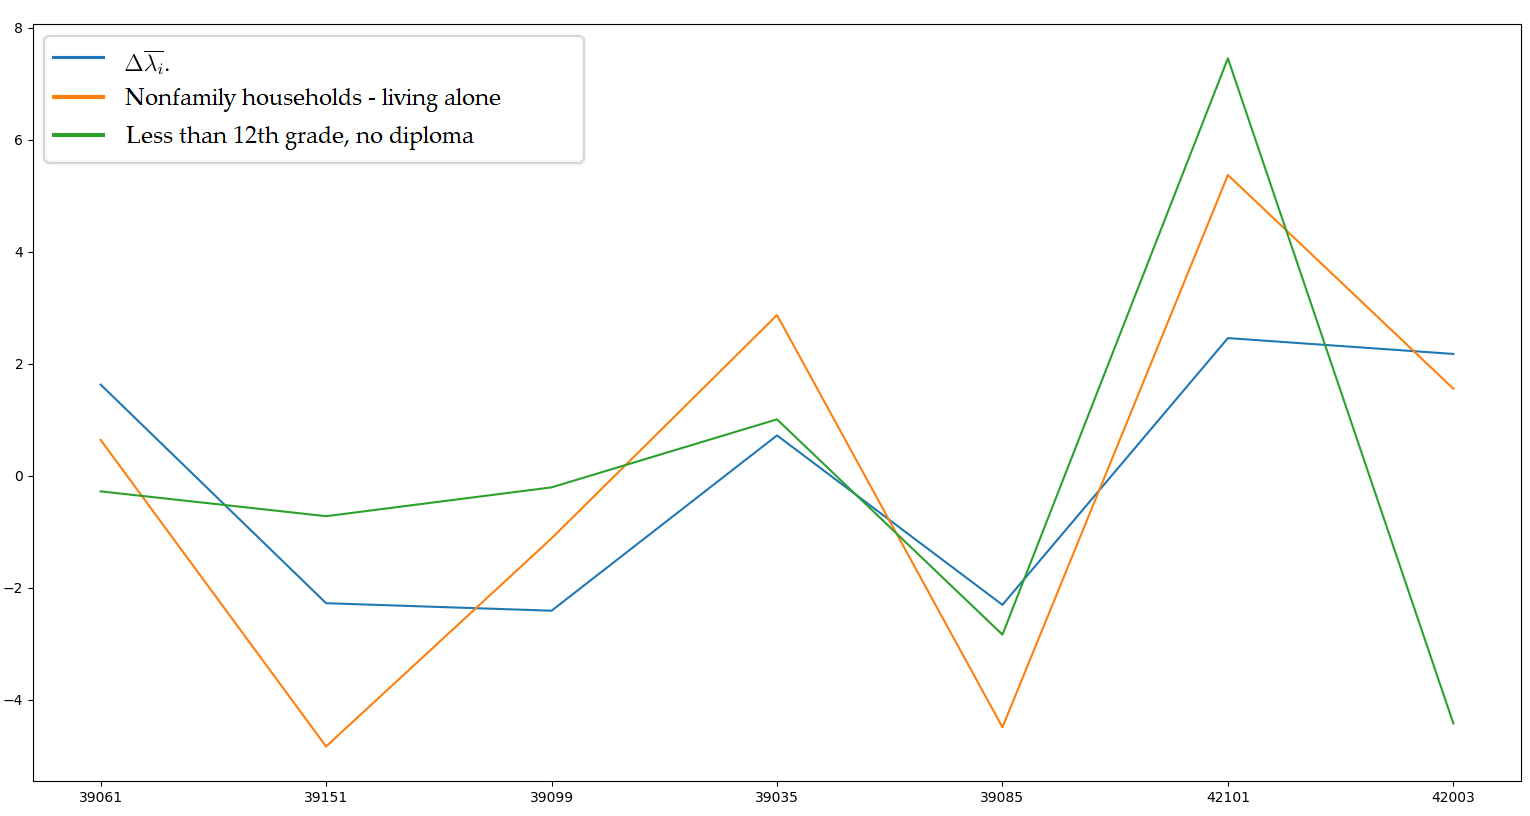
\includegraphics[width=0.7\linewidth]{005}
	\caption{the relationship between $\Delta \overline{\lambda_i}$, $\Delta \overline{y_{1i}}$ and  $\Delta \overline{y_{2i}}$}
\end{figure}

The consistency of the three attributes shown in the figure powerfully corroborated that $\Delta \overline{\lambda_i}$, $\Delta \overline{y_{1i}}$ and  $\Delta \overline{y_{2i}}$ are indeed positively correlated as we stated above. Thus, we build a linear regression model to describe their relationship as
\begin{equation}
\Delta \overline{\lambda_i} = k_1 \Delta \overline{y_{1i}} + k_2 \Delta \overline{y_{2i}} + k_3
\end{equation}

The solution to equation (20) is
\begin{equation}
\left\{
\begin{array}{l}
k_1 = 0.0193 \\
k_2 = 0.0319 \\
k_3 = -1.5340 \times 10^{-16} \\
\end{array}
\right.
\end{equation}
with coefficient of determination
\begin{equation}
R^2 = 0.9038
\end{equation} 

In the same way, we can also obtain the relationship between $\lambda_i$, $y_{1i}$ and $y_{2i}$. 

\begin{equation}
\lambda_i = k_4 y_{1i}+ k_5 y_{2i} + k_6
\end{equation}

with the solution

\begin{equation}
\left\{
\begin{array}{l}
k_4 = 0.0193 \\
k_5 = 0.0319 \\
k_6 = -0.9004 \\
\end{array}
\right.
\end{equation}

In fact, mathematically, the only difference between equation (21) and (24) is their intercepts.
Equation (24) describes how socio-economic factors affect our Opoid Spread Model from a quantitative point of view. When the details of opoid amount is not available, we would still be able to estimate the Sources' $\lambda$ through socio-economic factors.




\section{Strategy for Countering the Opioid Crisis}
\subsection{Strategy Description}
Basing on the analysis and results of section 4 and 5, we are profoundly aware of the central role that Sources play in the whole Opioid Spread Model. Under the premises that the government management resources are limited, we hope to find an optimal strategy to maximize the control of opioid spread while minimize the government resources used. 

Therefore, the strategy we take should mainly focus on Sources. To be more specific, we plan to:
\begin{itemize}
	\item Sourcesforce the opioid investigation efforts in Source counties to decrease the amount of opioid storage $S(t)$.
	\item Intensify inspection and control of private vehicles passing through cross-county road, hoping to limit the amount of opioid transported from Sources to Consumers $T^{OUT}(t)$.
\end{itemize}

We make some adjustments on the existing Discrete Opioid Spread Model in order to simulate and quantify opioid spread. No additional information could reveal the precise relationship between  $S$ and $S'$. Intuitively, we assume that 
\begin{equation}
S'(t) = \delta S(t)
\end{equation}
where
\begin{equation}
\delta \sim U(0, 0.1)
\end{equation}

Corresponding to the strategy we proposed earlier, we add a storage control coefficient $\alpha$ and a transport control coefficient $\beta$, such that
\begin{comment}
\begin{equation}
\alpha S_i(t) - S_i'(t) = \lambda S_i(t) + \beta T_i^{OUT}(t), \alpha\in (0,1), \beta \in (1, +\infty)
\end{equation}
Combining (23-25), we have
\end{comment}
\begin{equation}
(1 - \lambda - \delta)\alpha S_i(t) = \beta T_i^{OUT}(t), \alpha\in (0,1), \beta \in (1, +\infty)
\end{equation}
We set $\alpha$ in a range of $(0,1)$ because we hope that the storage after control $\alpha S(t)$ is smaller than the original storage. Similarly, we set $\beta > 1$ in that an increase in $\beta$ causes a decrease in $T^{OUT}$ when the left side of the equation (28) is known.

Mathematically, we could combine $\alpha$ and $\beta$ into one parameter to simplify analysis:
\begin{equation}
\varphi = \frac{\alpha}{\beta}
\end{equation}
thus
\begin{equation}
 (1 - \lambda - \delta) \varphi S_i(t) = T_i^{OUT}(t), \varphi \in (0,1)
\end{equation}




To test the effectiveness of this strategy, we focus on how the change in $\alpha$ and $\beta$ influences storage.

\subsection{Evaluating the Strategy}
\subsubsection{Simulating Opioid Spread}

\begin{wrapfigure}[13]{r}{0.25\linewidth} % Inline image example
	\begin{center}
		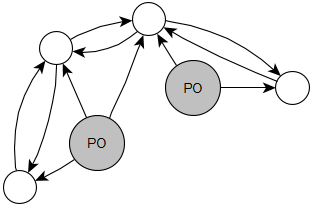
\includegraphics[width=\linewidth]{006}
	\end{center}
	\caption{Connection Between Sources and Others}
\end{wrapfigure}

We simulate opioid spread based on the directed graph we constructed in 4.2.1. We assume that drugs can be transported out of Sources into Consumers, but not vice versa. Thus we delete all edges pointing towards Sources in 4.2.1. 

We describe the simulation of opioid spread as:

\begin{enumerate}[(1)]
	\item At $t=0$, we initialize the diagram by setting the storage of Sources to $S_i(0)=\gamma_i$, where $\gamma_i>0$ is a constant for Source $i$. We construct set VISITED = $\emptyset$ and push all Sources into VISITED. We initialize an all-zero array S\_RECORD, with a mapping from node index to array index.
	
	\item At $t=k, k>0$, S\_RECORD is again set to zero and the storage of Sources to $S_i(0)=\gamma_i$. For all nodes in set VISITED, we calculate their opioid transportation to their out-neighbors using equation (9).For each node $i$, we add each $v_{ij}(t)$ to S\_Record[j]. After all nodes in the VISITED set were calculated, we add S\_Record[i] to $S_i$. After this, we traverse through the graph to add all nodes with $S>0$ but not yet in set VISITED into the set. 

\end{enumerate}

We compose a schematic diagram of storage flow. Inevitably, we will reach a point when all nodes are in the VISITED set. Simulation can carry on even when all nodes are visited. We visualize the spread in Figure 5:

\begin{figure}[H]
	\centering
	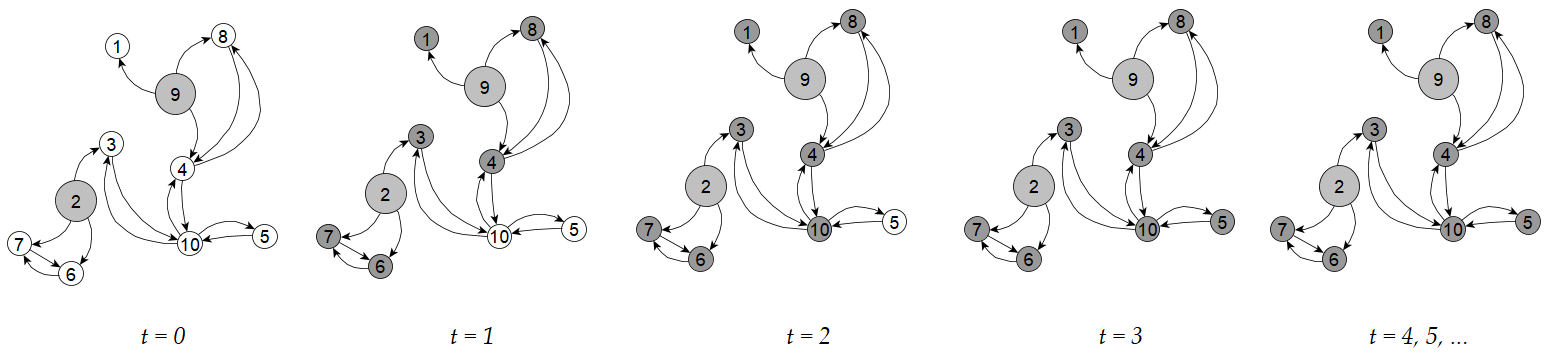
\includegraphics[width=\linewidth]{007}
	\caption{An Example Illustrating Opioid Spread Simulation. \textit{Node 2 and 9 are Sources. White nodes indiates nodes never visited. Gray nodes are nodes in VISITED set.}}
\end{figure}

We assume that in year 2017, we have reached a point where all nodes are visited. Therefore, we have only to consider the change in $S_i$ for each node $i$ with the increment of $t$. 

\subsubsection{Simulation Results}
We evaluate our strategy both qualitatively and quantatively. We take $\varphi = 0.4$ as an example.

Firstly, we compare the heatmap generated with that of non-control circumstances(i.e. $\varphi=1$). 

\begin{figure}[H]
	\centering
	\subfigure[$\varphi=1$]{
		\begin{minipage}[t]{0.45\linewidth}
			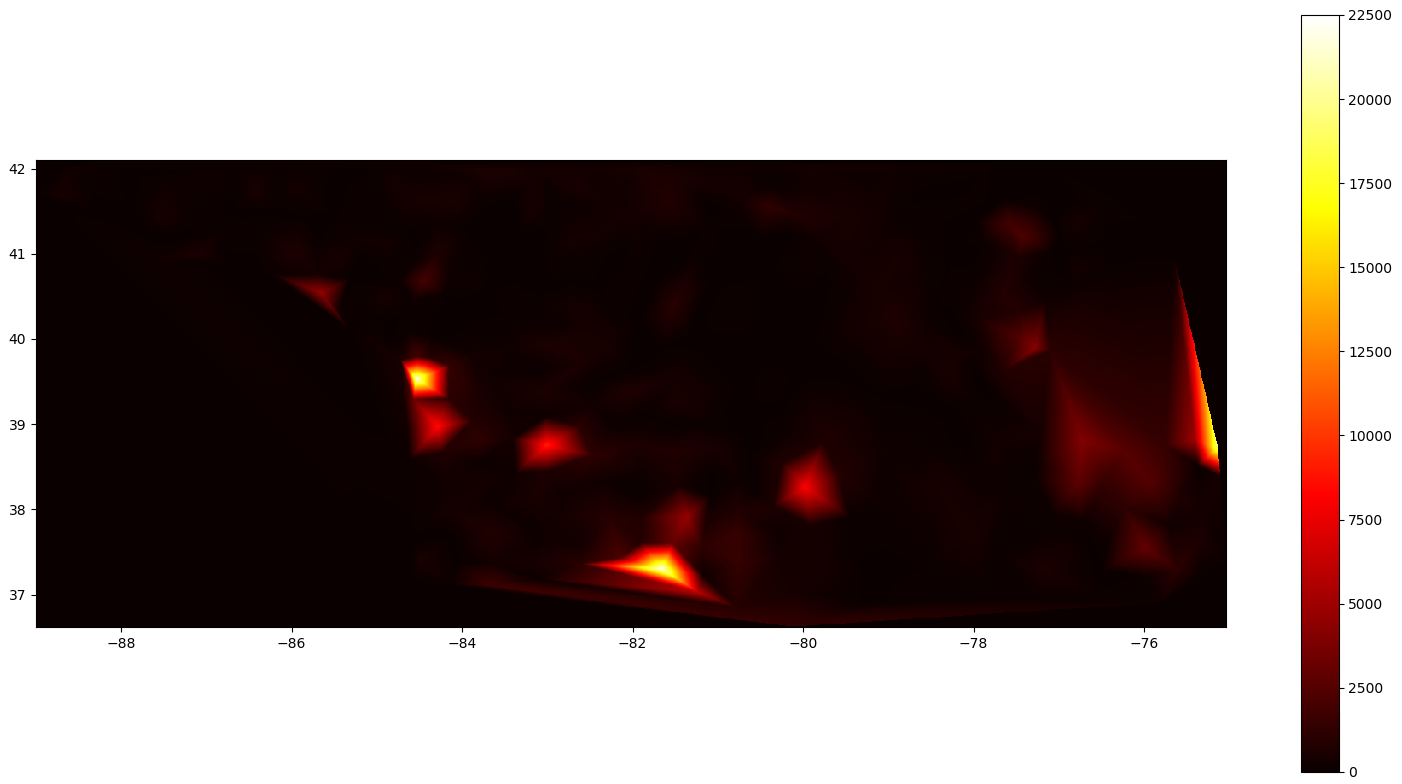
\includegraphics[width=\linewidth]{009}
		\end{minipage}
	}
	\subfigure[$\varphi=0.4$]{
		\begin{minipage}[t]{0.45\linewidth}
			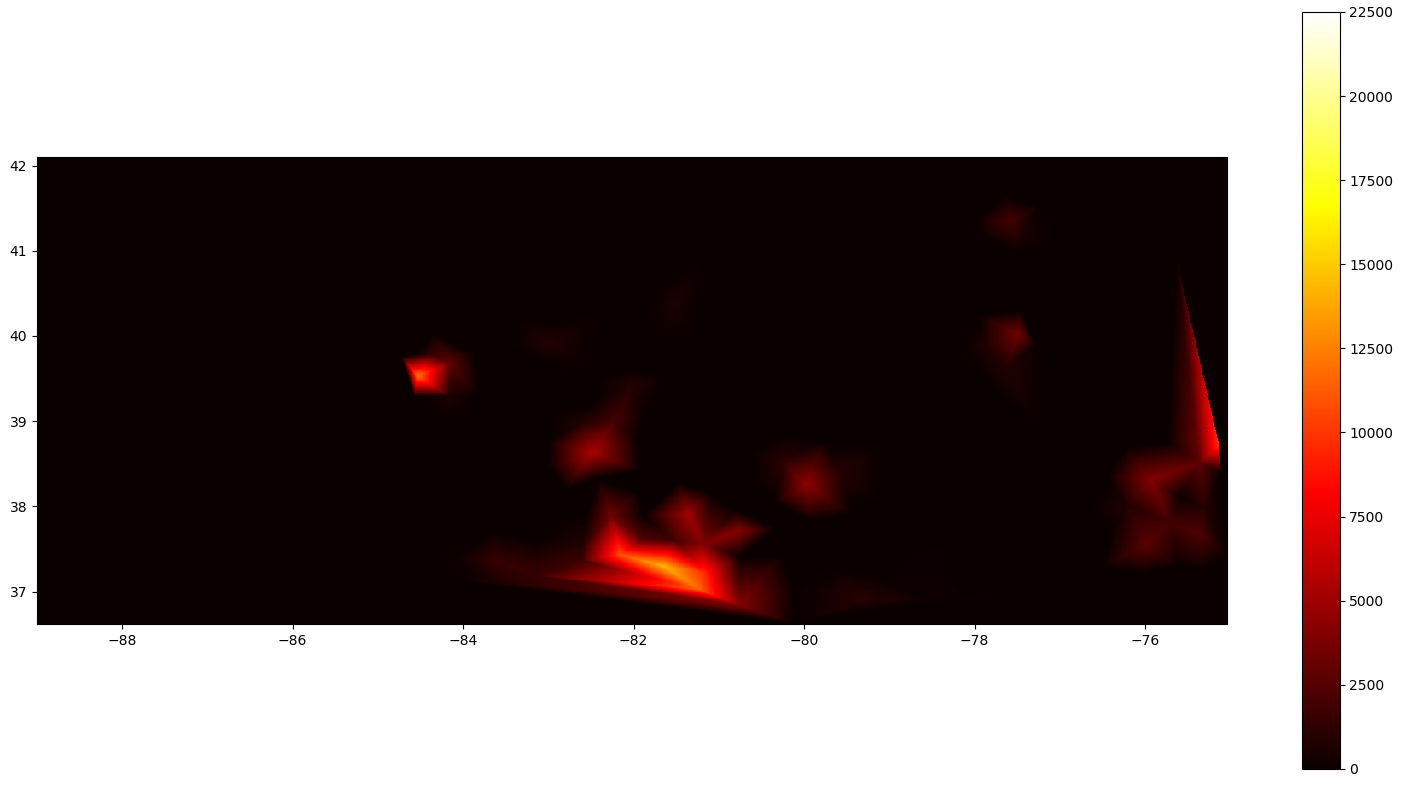
\includegraphics[width=\linewidth]{010}
		\end{minipage}
	}
	\caption{Heat Map Comparison}
\end{figure}
	
Secondly, let $n$ be the number of counties ranked second-level Sources and above. We compose a diagram of how $n$ changes over time. 

\begin{figure}[H]
	\centering
	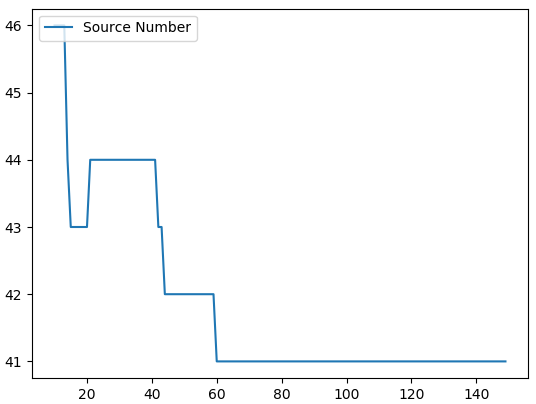
\includegraphics[width=0.3\linewidth]{011}
	\caption{n-t diagram}
\end{figure}

From the heatmap comparison(Figure 6), we reach the conclusion that the overall level of opioid storage declines dramatically. From the n-t Diagram(Figure 7), we can see that the number of Source counties decreased to some extent. 

%	\item Quantitative Method: using the threshold we proposed in Table Four, we hope that by controlling $\alpha$ and $\beta$, we could effectively reduce the number of first-level Sources and second-level Sources. Therefore, we define an ideal threshold $\mathcal{T}_1, \mathcal{T}_2$ to indicate an ideally low amount of first/second-level Sources, and compare how much time it takes for storage to change from the status in 2017 to our expected $\mathcal{T}_1, \mathcal{T}_2$ based on varying $\alpha$ and $\beta$. 
	
%	\item Qualitative Method: we generate a heat map of opioid storage at each time step $t$. Comparing these maps, we shall see the use-trend of opioids.


\subsection{Sensitivity Analysis: Identifing Significant Parameter Bounds}

We set simulation time long enough to observe how the number of Sources 
change over $\varphi$. As the scattered n-$\varphi$ diagram is shown below, the larger $\varphi$ is, the smaller $n$.

\begin{figure}[H]
	\centering
	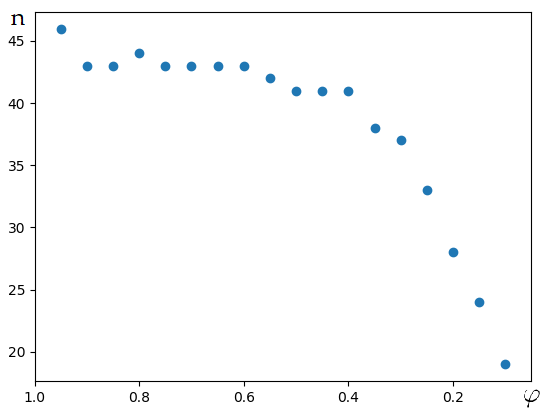
\includegraphics[width=0.3\linewidth]{008}
	\caption{n-$\varphi$ Diagram}
\end{figure}

From the diagram above, we observe that when $\varphi > 0.4$, the decrease in $n$ is relatively slow. However, a steep decrease occur when $\varphi < 0.4$. Thus, we suggest that the significant parameter(i.e. $\varphi$) bound is $0.4$.

\subsection{Extended Model}
To make the simulation of opioid spread closer to reality, we recommend some operations to improve the model, which are unnecessary in rough simulations.
\begin{enumerate}
	\item In our simulation process, we assume the Sources' storage $S(t)$ for each period $[t,t+1)$ to be a constant value. However, when control policies are functioning effectively, $S(t)$ is likely to be a gradually declining variable. We could define a decline coefficient to describe this scenario.
	
	\item Similar to what we analyzed for $S(t)$, when control strategies come into effect, the opioid consumption coefficient $\lambda$ would decline to some degree.
\end{enumerate}

However, we must keep in mind that a reasonable description of the declining process for the two coefficients stated above is no easy work.


\section{Conclusion}
\subsection{Conclusions}
We proposed a Opioid Spread Model to illustrate the spread and characteristics of the reported opioid crisis. Our model is promising for the following reasons:
\begin{enumerate}
	\item In order to adapt to different requirements, we constructed a complete set of analytical Opioid Spread Model through rigorous reasoning, including both Continuous and Discrete patterns. 
	
	\item Our model is precise and easy to understand. Simulation proved that it is easy to apply to reality.
	
	\item We quantified the relationship between $\lambda$ and socio-economic features, making it possible to estimate $\lambda$ with sociology statistics.
	
	\item We proposed a threshold for the government to distribute limited management resources to control opioid use based on former statics on opioid amount.
\end{enumerate}

\subsection{Limitations and Possible Solutions}
Even though our model successfully illustrated some features of opioid spread, it still possesses the following defects:
\begin{enumerate}
	\item Our analysis of a Source is only limited to an independent county, without considering the possibility that there may exist a region consisting of several neighboring counties with similar contributions to opioid amount. In other words, we failed to consider Source Regions consisting of several nodes.
	
	\item  In our simulation process, we neglected the possibility that a Source may become a Consumer and vice versa. The whole proceidure was based on the Origins but not other Sources.
	
	\item  When analyzing how socio-economic factors influence $\lambda$, lots of promising data were missing in the provided dataset. As a result, we were only able to extract two factors(i.e. education and loneliness). Even though we fully considered the independence among different factors, it may still exert a negative influence on the fitting precision. 
\end{enumerate}





\newpage
\section{Memorandum}
\textbf{To: }Chief Administrator, DEA/NFLIS Database \\
\textbf{From: }Team \# 1901279 \\
\textbf{Subject: }Strategy for Countering the Opidium Crisis \\
\textbf{Date: }January 26th, 2019\\
\rule{\textwidth}{0.1mm}
There is an impending crisis of opioid use owing to the alarming increase of opioid prescription and its widespread use and misuse. To address this crisis, our team propose a partial differential model to depict and analyze the spread of opioid use and its characteristics. Data from NFLIS and U.S. Census Beareau were used to simulate and test this model.

Our partial differential model, which was inspired by the Porous Media Contaminant Transport Model, implies the relationship between 

%----------------------------------------------------------------------------------------
%	BIBLIOGRAPHY
%----------------------------------------------------------------------------------------
\newpage
\begin{thebibliography}{99} % Bibliography - this is intentionally simple in this template

\bibitem{1}
Rummans, Teresa A., M. Caroline Burton, and Nancy L. Dawson. "How good intentions contributed to bad outcomes: the opioid crisis." \textit{Mayo Clinic Proceedings.} Vol. 93. No. 3. Elsevier, 2018.

\bibitem{2}
Overdose deaths involving opioids by type of opioid, United States, 2000-2015. From  \textit{CDC/NCHS National Vital Statistics System, Mortality}

\bibitem{3}
Bear J. Modeling Phenomena of Flow and Transport in Porous Media[M]. Springer, 2018.

\bibitem{4}
https://en.wikipedia.org/wiki/Lasso\_(statistics)

\bibitem{5}
Friedman, Jerome, Trevor Hastie, and Robert Tibshirani. The elements of statistical learning. Vol. 1. No. 10. New York, NY, USA:: Springer series in statistics, 2001.

\bibitem{6}
Friedman, Jerome, Trevor Hastie, and Rob Tibshirani. "Regularization paths for generalized linear models via coordinate descent." Journal of statistical software 33.1 (2010): 1.

\bibitem{7}
Kim, Seung-Jean, et al. "An Interior-Point Method for Large-Scale $\ell_1 $-Regularized Least Squares." IEEE journal of selected topics in signal processing 1.4 (2007): 606-617.

\bibitem{8}
Tang, D. H., E. O. Frind, and Edward Allan Sudicky. "Contaminant transport in fractured porous media: Analytical solution for a single fracture." Water resources research 17.3 (1981): 555-564.

\bibitem{9}
Burns, Lucy. "World Drug Report 2018 By United Nations Office on Drugs and Crime New York: United Nations, 2018.

\bibitem{10}
https://americanaddictioncenters.org/rehab-guide/addiction-statistics

\bibitem{11}
https://www.mayoclinic.org/diseases-conditions/prescription-drug-abuse/in-depth/how-opioid-addiction-occurs/art-20360372

\bibitem{12}
Hsu L C. Applying the grey prediction model to the global integrated circuit industry. Technological Forecasting and Social Change, 2003, 70(6): 563-574.

\bibitem{13}
https://www.census.gov/geo/reference/county-adjacency.html

\bibitem{14}
https://www.census.gov/geo/reference/ansi.html

\end{thebibliography}

%----------------------------------------------------------------------------------------
\newpage
\begin{comment}
\appendix
\appendixpage
\section{Mathematical Backgrounds}
\newpage
\section{EXAMPLES(TO BE DELETED!)}
% use http://www.tablesgenerator.com/latex_tables
\begin{table}[H]
	\centering
	\begin{tabular}{@{}llr@{}}
		\toprule
		\toprule
		\multicolumn{2}{c}{Item} &            \\ \cmidrule(r){1-2}
		Animal     & Description & Price (\$) \\ \midrule \midrule
		Gnat       & per gram    & 13.65      \\
		& each        & 0.01       \\
		Gnu        & stuffed     & 92.50      \\
		Emu        & stuffed     & 33.33      \\
		Armadillo  & frozen      & 8.99       \\ \bottomrule
	\end{tabular}
	\caption{My caption}
	\label{my-label}
\end{table}

\begin{figure}[H] % Example image
	\center{
\includegraphics[width=0.5\linewidth]{placeholder}}
	\caption{Example image.}
	\label{fig:speciation}
\end{figure}

\lipsum[6] % Dummy text
\begin{wrapfigure}{l}{0.4\textwidth} % Inline image example
	\begin{center}
		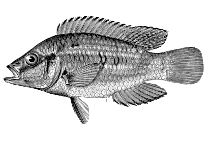
\includegraphics[width=0.38\textwidth]{fish}
	\end{center}
	\caption{Fish}
\end{wrapfigure}
\lipsum[7-8] % Dummy text

\begin{figure}[H]
	\centering
	\subfigure[Original]{
		\begin{minipage}[t]{0.25\linewidth}
			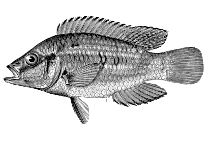
\includegraphics[width=1.4in]{fish}
		\end{minipage}
	}
	\subfigure[SIFT Features]{
		\begin{minipage}[t]{0.25\linewidth}
			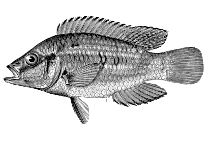
\includegraphics[width=1.4in]{fish}
		\end{minipage}
	}
	\caption{Source Image}
\end{figure}

\begin{description} % Numbered list example
	
	\item[First] \hfill \\
	\lipsum[9] % Dummy text
	
	\item[Second] \hfill \\
	\lipsum[10] % Dummy text
	
	\item[Third] \hfill \\
	\lipsum[11] % Dummy text
	
\end{description} 


%ALGORITHMS
\IncMargin{1em}
\LinesNumbered
\begin{algorithm}[H]
	\SetKwData{Left}{left}\SetKwData{This}{this}\SetKwData{Up}{up}
	\SetKwFunction{Union}{Union}\SetKwFunction{FindCompress}{FindCompress}
	\SetKwInOut{Input}{input}\SetKwInOut{Output}{output}
	
	\KwData{this text}
	\KwResult{how to write algorithm with \LaTeX2e }
	
	
	\BlankLine
	\While{not at end of this document}{
		read current\;
		\eIf{understand}{
			go to next section\;
			current section becomes this one\;
		}{
			go back to the beginning of current section\;
		}
	}
	\caption{How to write algorithms}
	
\end{algorithm}
\DecMargin{1em}
	
\end{comment}

\end{document}